%!TEX program = xelatex
\documentclass[11pt, a4paper]{article}
  \usepackage[a4paper,top=3cm,bottom=4cm,left=2.5cm,right=2.5cm]{geometry}
  \usepackage{subfig}
  \usepackage{graphicx}
  \graphicspath{{../images/}}
  \usepackage{hyperref}
  \usepackage{amsmath}
  \usepackage{braket}
  \usepackage{enumitem}
  \usepackage{mathtools}
  \usepackage{xepersian}
  \settextfont[Scale=1.2]{B Nazanin}
  \setlatintextfont[Scale=1]{Times New Roman Cyr}
  \title{\textbf{شبیه‌سازی رایانه‌ای در فیزیک}\\تمرین پنجم: تولید اعداد کاتوره‌ای}
  \author{سینا معمر ۹۵۱۰۲۳۱۶}
    

\begin{document}

\maketitle
\thispagestyle{empty}


\section{\textbf{مولد اعداد کاتوره‌ای}}
کد این بخش از تمرین را در فایل
\lr{q1.py}
می‌توان مشاهده نمود.
برای این کار‌ باید تابع
\lr{test\_randomness}
را با طول‌های دل‌خواه صدا بزنیم.
روش کار این تابع به این صورت است به تعداد بیش‌ترین طول داده شده، عدد تصادفی صحیح بین ۰ تا ۹ تولید می‌کند.
سپس بر روی لیست طول‌های داده شده پیمایش کرده و به تعداد آن طول، عدد از لیست اعداد تصادفی‌مان
بر می‌دارد و تعداد تکرار هر عدد را می‌شمارد.
سپس انحراف نسبی اعداد به دست‌ آمده را محاسبه کرده و در یک لیست جدید ذخیره می‌کند.
در آخر نیز آن را رسم می‌کند و شیب بهترین خط فیت شده به آن را به دست می‌آورد.
نتایج به دست آمده را در شکل‌های
\ref{fig:q1_histogram}
و
\ref{fig:q1_sigma}
می‌توان مشاهده نمود.
\\
همان طور که در شکل‌
\ref{fig:q1_histogram}
دیده می‌شود، در تعداد بالا پراکندگی اعداد بسیار نزدیک بهم است و از مقدار
$\frac{N}{10}$
انحراف چندانی ندارد.
همچنین می‌توان در شکل‌
\ref{fig:q1_sigma}
مشاهده نمود که انحراف نسبی با 
$\frac{1}{\sqrt{N}}$
رابطه‌ی مستقیم دارد. شیب خط فیت شده در این شکل برابر است با:
\begin{equation}
  \alpha = -0.486 \pm 0.001
\end{equation}

\begin{figure}[h!]
	\centering
  \begin{minipage}[b]{0.48\textwidth}
    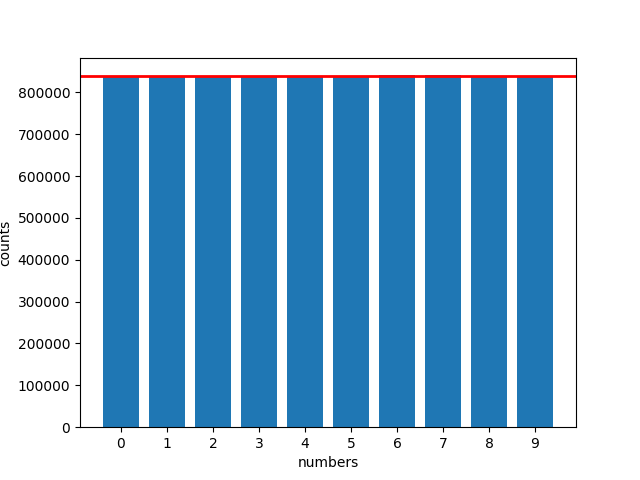
\includegraphics[width=\textwidth]{q1_histogram_14_24_2.png}
    \caption{پراکندگی اعداد تصادفی تولید شده با طول $2^{23}$}
    \label{fig:q1_histogram}
  \end{minipage}
  \hfill
  \begin{minipage}[b]{0.48\textwidth}
    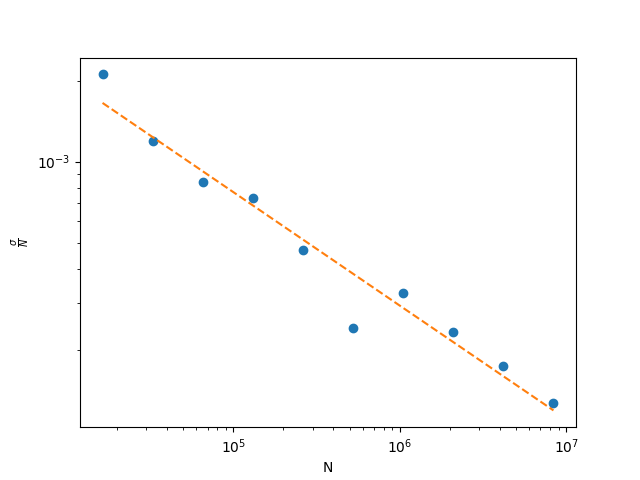
\includegraphics[width=\textwidth]{q1_sigma_14_24_2.png}
    \caption{تغییرات انحراف نسبی بر حسب $N$}
    \label{fig:q1_sigma}
  \end{minipage}
\end{figure}

در ول‌نشست نیز همانند این مسئله،
$\sigma^2 \sim N$
است.
علت این موضوع این است که این مسئله کاملا معادل با یک مسئله‌ی ول‌نشست به طول ۱۰ است.
در آن جا نیز ما باید به طور تصادفی از بین مجموعه‌ای از اندیس‌ها انتخاب می‌کردیم و
با هر انتخاب طول آن دسته یکی افزایش پیدا می‌کرد.
به همین دلیل رفتار ول‌نشست کاملا مشابه با رفتار تولید اعداد تصادفی است.


\section{\textbf{هم‌بستگی}}
کد این بخش از تمرین را در فایل
\lr{q2.py}
می‌توان مشاهده نمود.
برای این کار باید تابع
\lr{test\_correlation}
را با عدد‌ و طول دل‌خواه صدا کنیم.
روش کار این تابع کاملا مشابه با تمرین اول است،
تنها با این تفاوت که پراکندگی و انحراف و نسبی را برای عدد‌های تصادفی‌ای که بعد از عدد داده شده می آیند،
محاسبه می‌کنیم.
نتایج به دست آمده را برای عدد
$4$
در شکل‌های
\ref{fig:q2_histogram}
و
\ref{fig:q2_sigma}
می‌توان مشاهده نمود.
همان‌طور که مشاهده می‌شود، فراوانی این اعداد بسیار نزدیک به
$\frac{N}{100}$
می‌باشد که مطابق با انتظار ما نیز است.
شیب خط فیت شده نیز برابر با:

\begin{equation}
  \alpha = -0.498 \pm 0.001
\end{equation}

که مطابق با انتظار ما است.

\begin{figure}[h!]
	\centering
  \begin{minipage}[b]{0.48\textwidth}
    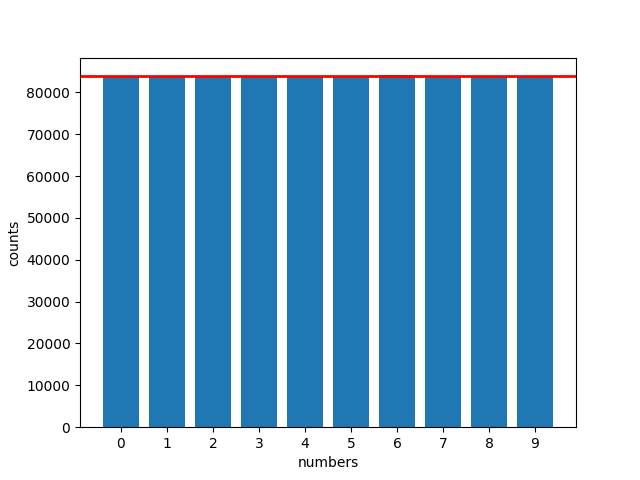
\includegraphics[width=\textwidth]{q2_histogram_4_14_24_2.png}
    \caption{پراکندگی اعداد تصادفی بعد از عدد $4$ به طول $10^7$}
    \label{fig:q2_histogram}
  \end{minipage}
  \hfill
  \begin{minipage}[b]{0.48\textwidth}
    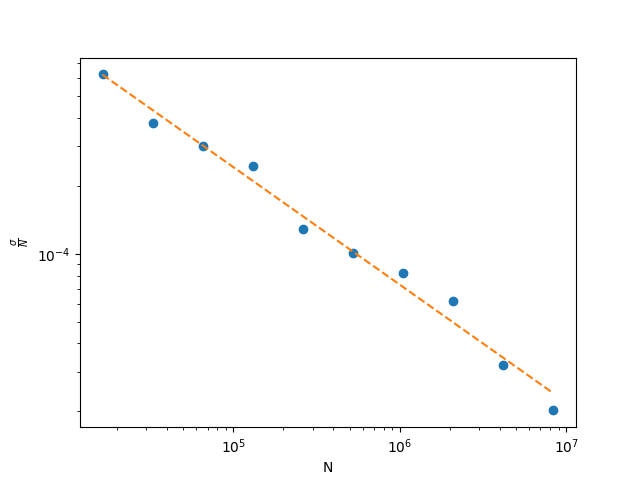
\includegraphics[width=\textwidth]{q2_sigma_4_14_24_2.png}
    \caption{تغییرات انحراف نسبی بر حسب $N$ برای اعداد پس از $4$}
    \label{fig:q2_sigma}
  \end{minipage}
\end{figure}


\section{\textbf{قضیه‌ی حد مرکزی}}
کد این بخش از تمرین را در فایل
\lr{q3.py}
می‌توان مشاهده نمود.
برای این کار باید تابع
\lr{test\_central\_limit}
را با عدد‌ها و تعداد نمونه‌های دل‌خواه صدا بزنیم.
روش کار این تابع به این شکل است که 
روی عدد‌های داده شده پیمایش کرده و به تعداد نمونه‌های داده شده، بسته‌هایی به تعداد عدد داده شده از اعداد تصادفی
بین ۰ تا ۹ تولید کرده و جمع هر کدام از این بسته‌ها را محاسبه می‌کند.
در نهایت نیز پراکندگی این جمع‌های به دست آمده را رسم می‌کند.
نتایج به دست آمده را در شکل‌های
\ref{fig:q3_5}
تا
\ref{fig:q3_1000}
می‌توان مشاهده نمود.
همان طور که مشاهده می‌شود، نتایج به دست آمده کاملا با توزیع گاوسی هم‌خوانی دارند و از آن پیروی می‌کنند.

\begin{figure}[h!]
	\centering
  \begin{minipage}[b]{0.48\textwidth}
    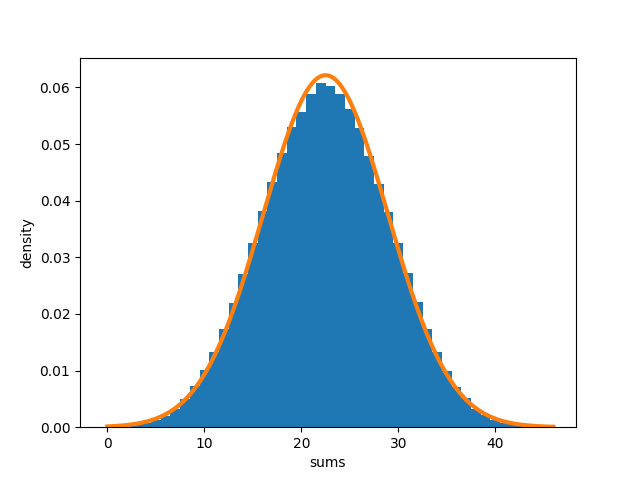
\includegraphics[width=\textwidth]{q3_5_1000000.png}
    \caption{پراکندگی‌ جمع $5$ عدد با $10^6$ نمونه}
    \label{fig:q3_5}
  \end{minipage}
  \hfill
  \begin{minipage}[b]{0.48\textwidth}
    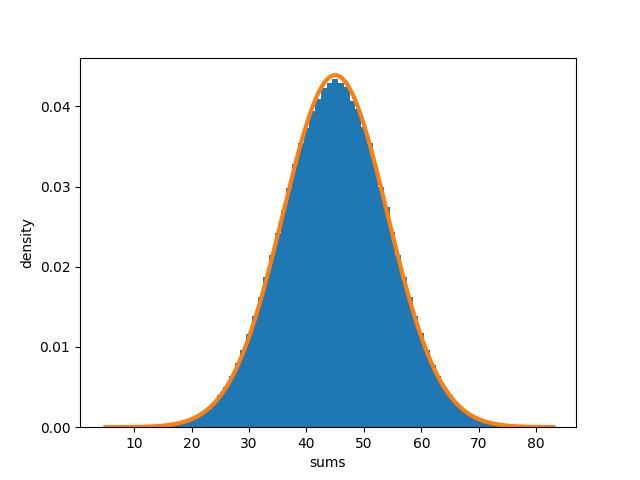
\includegraphics[width=\textwidth]{q3_10_1000000.png}
    \caption{پراکندگی‌ جمع $10$ عدد با $10^6$ نمونه}
    \label{fig:q3_10}
  \end{minipage}
  \begin{minipage}[b]{0.48\textwidth}
    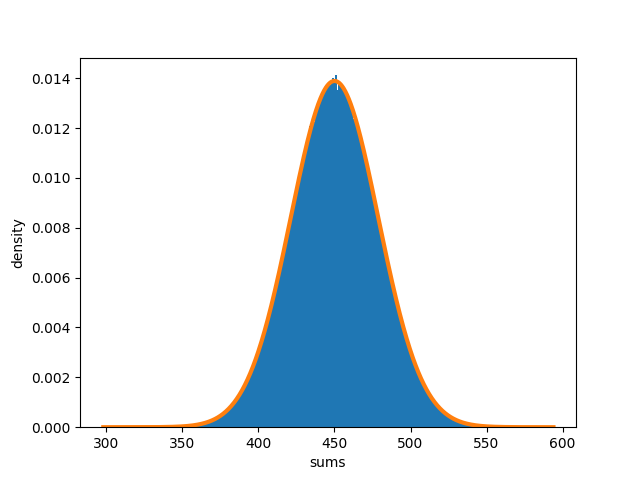
\includegraphics[width=\textwidth]{q3_100_1000000.png}
    \caption{پراکندگی‌ جمع $100$ عدد با $10^6$ نمونه}
    \label{fig:q3_100}
  \end{minipage}
  \hfill
  \begin{minipage}[b]{0.48\textwidth}
    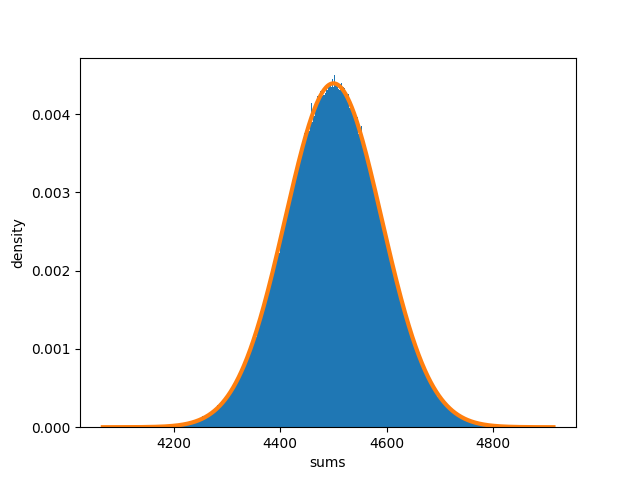
\includegraphics[width=\textwidth]{q3_1000_1000000.png}
    \caption{پراکندگی‌ جمع $1000$ عدد با $10^6$ نمونه}
    \label{fig:q3_1000}
  \end{minipage}
\end{figure}

این تمارین کاملا مشابه یکدیگر هستند از این جهت که می‌توان آن‌ها را تبدیل به هم‌دیگر کرد.
در ول‌گشت ما در هر مر‌حله به طور تصادفی یک عدد از بین
$1$
و
$-1$
انتخاب می‌کردیم و آن را به قدم‌های قبلی اضافه می‌کردیم.
در این‌جا نیز داریم مشابه همان کار را انجام می‌دهیم.
به این صورت که گام‌هایمان به طول
$0$
تا
$9$
هستند و احتمال‌شان نیز برابر است.
پس توزیع مکان‌های یک مسئله‌ی ول‌گشت در مرحله‌ی
\lr{t}
باید مشابه با توزیع جمع
\lr{t}
عدد تصادفی باشد.
در مورد مسئله‌ی ول‌نشست نیز به همین صورت است.
گام‌هایمان به طول‌
$0$
و
$1$
هستند و احتمال گام‌ها
$0$،
$9$
برابر احتمال گام
$1$
است.
پس طول دسته‌های ول‌نشت نیز باید توزیعی مشابه با جمع اعداد تصادفی داشته باشد.


\section{\textbf{تغییر تابع توزیع}}
کد این بخش از تمرین را در فایل
\lr{q4.py}
می‌توان مشاهده نمود.
برای این کار باید تابع
\lr{gaussian\_random\_ generator}
را با انحراف معیار و تعداد دل‌خواه فراخوانی کنیم.
روش کار این تابع به این صورت است که به تعداد داده شده، جفت اعداد تصادفی با توزیع یک‌نواخت تولید می‌کند.
سپس با توجه به رابطه‌ای که برای تبدیل داریم،
این جفت اعداد را به یک مختصات قطبی تبدیل کرده و از روی آن دو عدد تصادفی با توزیع گاوسی به دست می‌آوریم.
نتایج به دست آمده را در شکل‌
\ref{fig:q4}
می‌توان مشاهده نمود.
همان طور که دیده می‌شود رفتار آن کاملا از توزیع گاوسی پیروی می‌کند.

\begin{figure}[h]
  \centering
  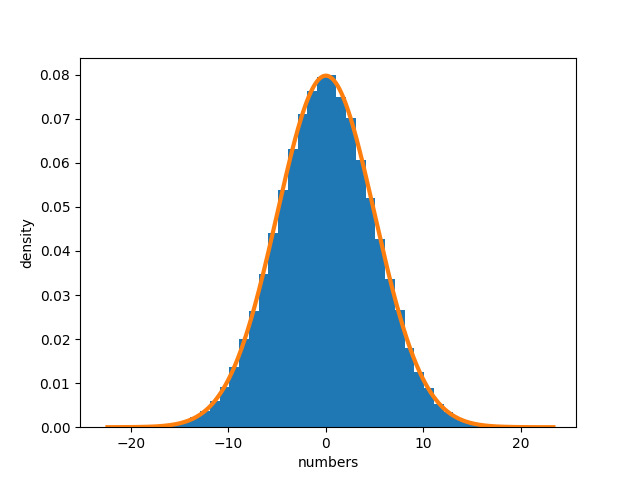
\includegraphics[width=.7\textwidth]{q4_5_100000.png}
  \caption{پراکندگی اعداد تصادفی با توزیع گاوسی ساخته شده از توزیع یکنواخت برای $200\,000$ عدد}
  \label{fig:q4}
\end{figure}


\end{document}
